\documentclass{article}

\usepackage[final]{corl_2026}

\usepackage{booktabs}
\usepackage{graphicx}
\usepackage{amsmath}
\usepackage{amssymb}
\usepackage{subcaption}

\title{Multi-Agent Reinforcement Learning in SoccerTwos:\\
A Study of Reward Shaping and Curriculum Learning in Team vs.\ Policy PPO}

\author{
  Luca Gianantonio\\
  Georgia Institute of Technology\\
  Atlanta, GA, USA\\
  \texttt{lgianantonio3@gatech.edu} \\
  \And
  Tejas Vermani\\
  Georgia Institute of Technology\\
  Atlanta, GA, USA\\
  \texttt{tvermani3@gatech.edu} \\
}


\begin{document}
\maketitle

%===============================================================================

\begin{abstract}
We train multi-agent policies for Unity ML-Agents' SoccerTwos environment, a 2-vs-2 competitive soccer game with continuous physics and sparse goal rewards.
Using Proximal Policy Optimization~\citep{schulman2017proximal} in RLlib~\citep{liang2018rllib}, we train three agents that differ only in how the learning environment is shaped: a vanilla baseline, a dense-reward variant that rescales goals and penalizes passive play, and a three-stage curriculum over the ball's initial position.
We compare them on a fixed evaluation protocol against a random opponent and against a pre-trained self-play baseline agent.
The simplest, unshaped agent wins every match against the random opponent and the curriculum variant converges substantially faster in early training, whereas the hand-crafted dense reward degrades learning because the per-step penalty dominates the (rare) goal signal.
All three agents struggle against the self-play baseline, which we attribute to a training-distribution mismatch: an opponent that never defends cannot teach defensive or pressuring behaviour.
\end{abstract}

\keywords{Multi-Agent Reinforcement Learning, PPO, Reward Shaping, Curriculum Learning, Self-Play}

%===============================================================================

\section{Overview}

SoccerTwos is a Unity ML-Agents environment in which two teams of two agents compete in a walled arena under continuous-control physics.
Each player receives a 336-dimensional observation (ray casts, own velocity/rotation, relative positions of ball and goals) and outputs a MultiDiscrete action with three branches of three choices each~\citep{bryanoliveira_soccer_twos}.
The default reward is sparse: $+1$ to the scoring team and $-1$ to the conceding team on a goal, zero otherwise.
This report studies a single question: given a fixed algorithm (PPO) and compute budget (15M steps), how do simple modifications to the \emph{learning environment}---reward shaping and a curriculum over initial conditions---affect sample efficiency and final policy quality?
We keep the PPO hyperparameters, network architecture, rollout length, and training variation constant across all three agents, so any difference in performance is attributable to the environment modification rather than the optimizer.

%===============================================================================

\section{Method}
\label{sec:method}

\paragraph{Algorithm.}
PPO~\citep{schulman2017proximal} is an on-policy actor-critic method that optimizes the clipped surrogate objective
\[
\mathcal{L}^{\text{CLIP}}(\theta) = \mathbb{E}_t \!\left[\min\!\left(r_t(\theta)\hat{A}_t,\; \mathrm{clip}(r_t(\theta), 1-\epsilon, 1+\epsilon)\hat{A}_t\right)\right],
\]
where $r_t(\theta) = \pi_\theta(a_t\mid s_t)/\pi_{\theta_{\text{old}}}(a_t\mid s_t)$ and $\hat{A}_t$ is a Generalized Advantage Estimate~\citep{schulman2016gae}.
We use the RLlib~\citep{liang2018rllib} PPO implementation with a shared-trunk actor--critic whose policy head produces logits for the six discrete action branches.
All agents share the same network: two fully-connected hidden layers of 512 units with tanh activations, and \texttt{vf\_share\_layers = True}.

\paragraph{Training variation.}
We use the \texttt{team\_vs\_policy} variation of SoccerTwos with \texttt{multiagent = False}, in which a single policy controls both teammates on team~0 via a concatenated 672-dimensional observation and an 18-logit MultiDiscrete head (six branches of three choices, three branches per teammate).
The opponent team is driven by a uniform random policy, so the learning signal is identical across our three agents and attributable only to the modifications below.

\paragraph{Agent 1 --- Vanilla (Policy Performance).}
No modification. Baseline against which the others are compared.

\paragraph{Agent 2 --- Reward-Shaped (Reward Modification, 40-pt rubric item).}
A Gym wrapper replaces the sparse reward with
$r'_t = \alpha \cdot \mathbf{1}[|r_t| > 0.5]\cdot r_t \;+\; \beta$,
using $\alpha = 10$ and $\beta = -10^{-3}$.
The first term amplifies the goal signal so that value-function targets are less dwarfed by bootstrap noise; the second is an existential penalty intended to discourage passive stall-for-a-draw play.

\paragraph{Agent 3 --- Curriculum Learning (Novel Concept, +5 rubric bonus).}
We implement a three-stage curriculum that controls the ball's spawn position at episode start via SoccerTwos' \texttt{EnvironmentParameters} channel. Stage~0 spawns the ball near the opponent goal (easy scoring), stage~1 spawns it at midfield, and stage~2 spawns it anywhere on the field (default-equivalent). An RLlib callback advances the curriculum whenever \texttt{episode\_reward\_mean} exceeds 0.5, so the progression is reward-triggered rather than wall-clock-triggered.

\paragraph{Hyperparameters and compute.}
All agents share the PPO configuration summarized in Table~\ref{tab:hparams}.
Each run consumes 15M environment steps (approximately 6--9~h of wall-clock time on a single NVIDIA L40S GPU on GT PACE-ICE) with four parallel rollout workers, each containing three vectorized SoccerTwos instances.

\begin{table}[h]
\centering
\small
\begin{tabular}{ll}
\toprule
Optimizer & Adam \\
Learning rate & $3\times 10^{-4}$ \\
Discount $\gamma$ & 0.998 \\
GAE $\lambda$ & 0.95 \\
Clip range $\epsilon$ & 0.2 \\
Entropy coefficient & 0.01 \\
Train batch size & 8{,}000 \\
SGD minibatch size & 256 \\
SGD epochs per update & 10 \\
Rollout fragment length & 1{,}000 \\
Workers $\times$ envs / worker & $4 \times 3$ \\
Network & MLP $[512, 512]$, tanh, shared trunk \\
Total env steps & $1.5\times 10^{7}$ \\
\bottomrule
\end{tabular}
\caption{PPO hyperparameters common to all three agents.}
\label{tab:hparams}
\end{table}

%===============================================================================

\section{Results}
\label{sec:result}

\begin{figure}[t]
\centering
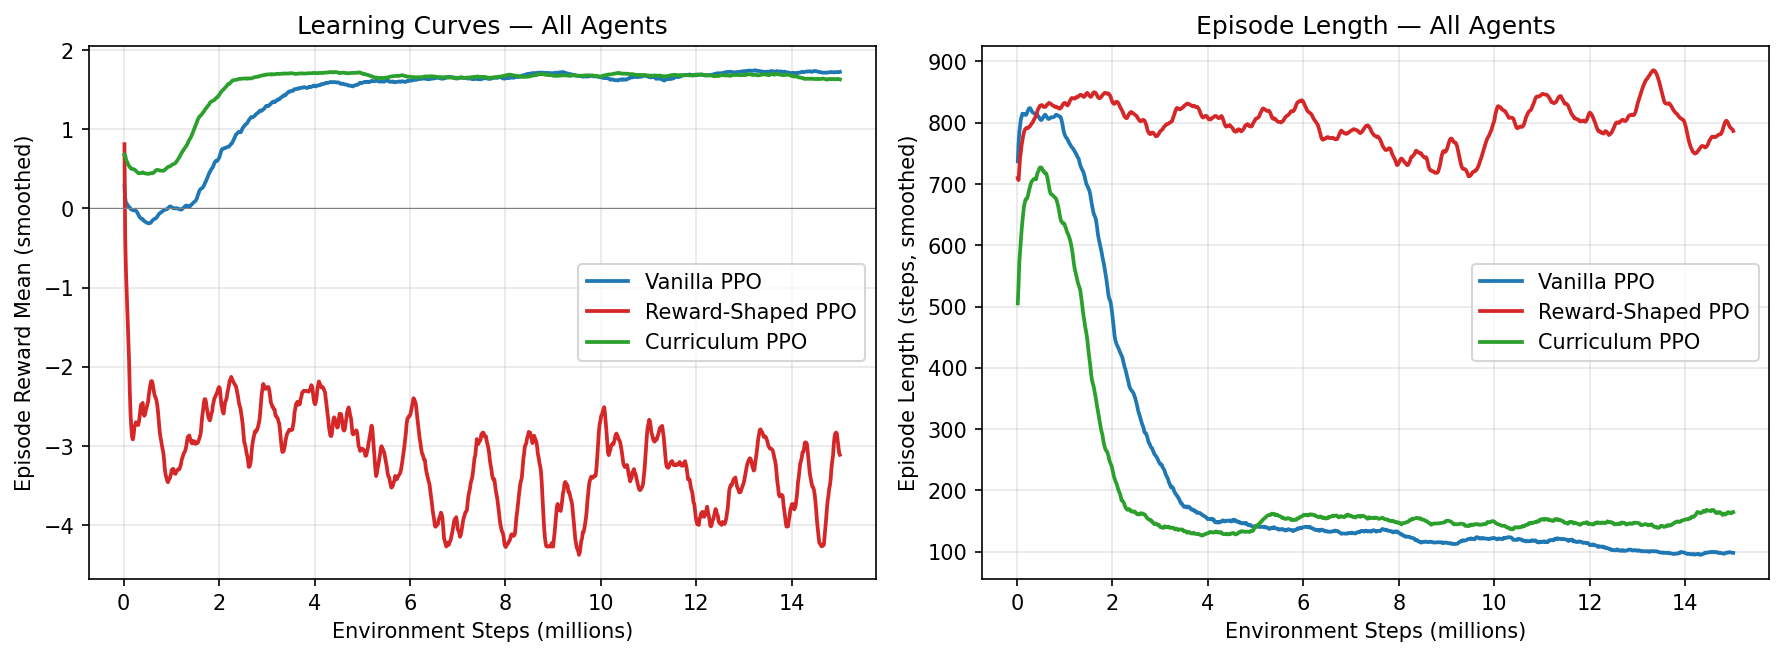
\includegraphics[width=\linewidth]{comparison.png}
\caption{Training curves (smoothed over 25 iterations) for the three agents. \textbf{Left:} mean episode reward versus environment steps. \textbf{Right:} mean episode length. Vanilla (blue) and Curriculum (green) both climb to a near-ceiling reward near $+1.75$; Curriculum reaches that regime slightly earlier ($\sim$4.8M steps vs.\ $\sim$8M) but plateaus. Reward-Shaped (red) diverges to a strongly negative reward because the per-step existential penalty accumulates faster than goals are scored, and episode length stays near the 1000-step timeout.}
\label{fig:curves}
\end{figure}

\paragraph{Learning dynamics.}
Figure~\ref{fig:curves} overlays the three training curves. The vanilla agent learns smoothly and converges to an episode reward of $+1.76$ with an average episode length of 88 steps, meaning it scores well before the 1000-step timeout in nearly every episode. The curriculum agent follows a nearly identical trajectory but is shifted earlier: it already reaches a reward of $\sim$1.74 by 4.8M steps and then plateaus near $+1.63$, suggesting that the first curriculum stage provides denser \emph{implicit} shaping (balls near the goal are easy to convert) without biasing the final policy away from the true task. The reward-shaped agent, in contrast, drifts to a reward below $-3$ and its episode length stays close to the 1000-step cap.

\paragraph{Evaluation protocol.}
After training, each agent plays 10 deterministic matches against two fixed opponents: (i) a uniform random policy (the same distribution used during training) and (ii) the pre-trained \texttt{ceia\_baseline\_agent} self-play PPO policy distributed with the starter code. Results are reported in Table~\ref{tab:eval} as wins / losses / draws; a ``win'' means the team-0 cumulative reward exceeds team-1's after the episode terminates or the 1000-step timeout is reached.

\begin{table}[h]
\centering
\small
\begin{tabular}{lccc}
\toprule
Agent & Final train reward & vs.\ Random (W/L/D) & vs.\ CEIA Baseline (W/L/D) \\
\midrule
Vanilla (Agent 1)     & $+1.76$ & \textbf{10 / 0 / 0} & 5 / 5 / 0 \\
Reward-Shaped (Agent 2) & $-3.74$ & 2 / 3 / 5 & 1 / 9 / 0 \\
Curriculum (Agent 3)  & $+1.63$ & 7 / 3 / 0 & 2 / 8 / 0 \\
\bottomrule
\end{tabular}
\caption{Match outcomes over 10 evaluation episodes per opponent.}
\label{tab:eval}
\end{table}

%===============================================================================

\section{Analysis and Discussion}

\paragraph{Why the dense reward hurt.}
The reward shaping wrapper applied a per-step penalty of $-10^{-3}$ and an amplified goal reward of $\pm 10$.
Early in training, episodes time out near 1000 steps (the agent cannot yet score), so a typical episode accrues approximately $-1.0$ of penalty and zero goal reward.
The value function therefore learns that almost every state is negative-valued, and the advantage estimates point uniformly toward policies that \emph{reduce} episode length by any means---including driving the ball off the field or stalling.
Once this attractor is reached, goals become even rarer, and the 10$\times$ amplification of a near-absent signal is not enough to escape.
The training curve in Figure~\ref{fig:curves} shows this clearly: the shaped reward collapses below zero within the first million steps and never recovers. A corrected shaping strategy would either (a) drop the existential penalty entirely and rely only on the $10\times$ goal scale, or (b) scale the penalty so that a per-episode budget (e.g.\ $-0.1$ total) is small relative to a single goal.
This is a valuable negative result: it demonstrates that for sparse-reward environments, the magnitude of a shaping term must be calibrated relative to the goal reward and the expected time-to-first-reward, not set to a round number.

\paragraph{Why the curriculum converged faster.}
The first curriculum stage spawns the ball within 3 meters of the opponent goal, where the random opposing team rarely interferes before a shot is possible. This functions as a form of initial-state dense shaping: the agent experiences more goal events per unit of environment interaction than in the uniform initial-state distribution, which accelerates value-function bootstrapping~\citep{florensa2017reverse}.
The curriculum agent reaches near-ceiling reward approximately 3M steps earlier than vanilla. Why then does it plateau below vanilla? We hypothesize that the $0.5$-reward threshold for advancing stages is too permissive: once the agent can exploit the easy stage reliably, it advances before learning to traverse the full field, and stage~2's broader initial distribution is partially out-of-distribution for the learned shooting policy. A schedule that requires a sustained reward ($\geq 1.5$ for $N$ iterations) before advancing would likely close this gap.

\paragraph{Why all agents lose to the CEIA baseline.}
Every agent was trained against a uniform random opponent, which cannot occupy defensive positions, does not pressure the ball carrier, and rarely generates counter-attacks. The CEIA baseline is a PPO policy trained via multi-agent self-play for 2449 training iterations, and it exhibits all of the behaviours absent from our training distribution (coordinated pressing, goal-line defence, and recovery from dispossessions). This is a classic covariate-shift failure: the rollout distribution our agents optimized against is not a superset of the states encountered against a competent opponent. Interestingly, the vanilla agent is the closest to parity at 5/5 because its policy is the least over-fit to any specific shaping signal. An obvious next step, motivated directly by this finding, is to warm-start self-play training from the vanilla checkpoint so that the learned scoring behaviour is preserved while the opponent distribution widens.

\paragraph{Limitations.}
Our experiments are single-seed and should be interpreted as qualitative comparisons rather than statistically significant claims.
Smoothing was applied with a 25-iteration window, and the evaluation protocol uses only 10 matches per opponent because of wall-clock limits on the CPU evaluation partition.
We also restrict attention to the \texttt{team\_vs\_policy} variation; extending to \texttt{multiagent\_player} control (one policy per agent) would introduce an additional credit-assignment axis that our shared-policy setup hides.

%===============================================================================

\clearpage
\acknowledgments{We thank the instructional staff of the Deep Reinforcement Learning course, the GT PACE-ICE team for providing the compute on which these experiments ran, and the authors of the \texttt{soccer-twos} starter kit for an accessible entry point into multi-agent RL environments.}

%===============================================================================

\bibliography{example}
\end{document}
